\chapter{Plots, Charts, \& Graphs}\label{ch:plotsandgraphs}
		Throughout this chapter we will be exploring some of the different ways of displaying your data in your thesis.
		Mainly this will be accomplished with the \pkg{pgfplots} package.
		In the following sections, there will be a few examples of how to generate different plots.
		For more information on how to create plots, \href{https://mirror.its.dal.ca/ctan/graphics/pgf/contrib/pgfplots/doc/pgfplots.pdf}{\textcolor{blue}{\underline{here}}} is the manual for \pkg{pgfplots}(the package used to generate the information for TikZ to create the plots).

	\section{Line Plots}
		A simple line plot can be effectively created using the \env{axis} environment from the \pkg{pgfplots} package in \LaTeX. 
		The \pkg{pgfplots} package is a powerful tool for creating high-quality plots directly within \LaTeX\ documents. 
		It builds upon the \pkg{TikZ} package and provides a comprehensive set of options for plotting and customizing graphs.

		The following code (see \Cref{lst:line-plot}) can be used to create the figure shown in \Cref{plt:line-plot}.
		\begin{figure}[!h]
		\centering
		\begin{subfigure}[b]{0.45\linewidth}
		\centering
		\begin{lstlisting}[style=LaTeXStyle,basicstyle=\scriptsize\ttfamily,frame=single]
\begin{figure}[htbp]
	\centering
	\begin{tikzpicture}
		\begin{axis}[
			title={Simple Line Plot},
			xlabel={X-axis},
			ylabel={Y-axis},
		]
			\addplot coordinates {
				(0,0)
				(1,1)
				(2,4)
				(3,9)
				(4,16)
			};
		\end{axis}
	\end{tikzpicture}
	\caption{A simple line plot.}
	\label{fig:line-plot}
\end{figure}
		\end{lstlisting}
		\caption{}
		\label{lst:line-plot}
		\end{subfigure}
		\hfill
		\begin{subfigure}[b]{0.45\linewidth}
			\centering
			\begin{tikzpicture}
				\begin{axis}[
					width=\linewidth,
					title={Simple Line Plot},
					xlabel={X-axis},
					ylabel={Y-axis},
				]
					\addplot coordinates {
						(0,0)
						(1,1)
						(2,4)
						(3,9)
						(4,16)
					};
				\end{axis}
			\end{tikzpicture}
			\caption{}
			\label{plt:line-plot}
		\end{subfigure}
			\caption[A simple line plot.]{A simple line plot (\subref{plt:line-plot}) and the code to generate the plot (\subref{lst:line-plot})}\label{fig:line-plot}
		\end{figure}
		Expanding on this example, we can add a second plot by adding the following code below the closing bracket and semi-colon (\texttt{\};}) of the \cmd{addplot} command:
		\begin{lstlisting}[float=ht,caption=,label=lst:line-plot-2,style=LaTeXStyle,basicstyle=\small\ttfamily,]
\addplot coordinates {
	(0,16)
	(1,9)
	(2,4)
	(3,1)
	(4,0)
};
		\end{lstlisting}
		This will result in the addition of the second red line shown in \Cref{fig:line-plot-2}.
		\begin{figure}[htbp]
			\begin{subfigure}[b]{0.45\linewidth}
				\centering
				\begin{lstlisting}[style=LaTeXStyle,basicstyle=\scriptsize\ttfamily,frame=single]
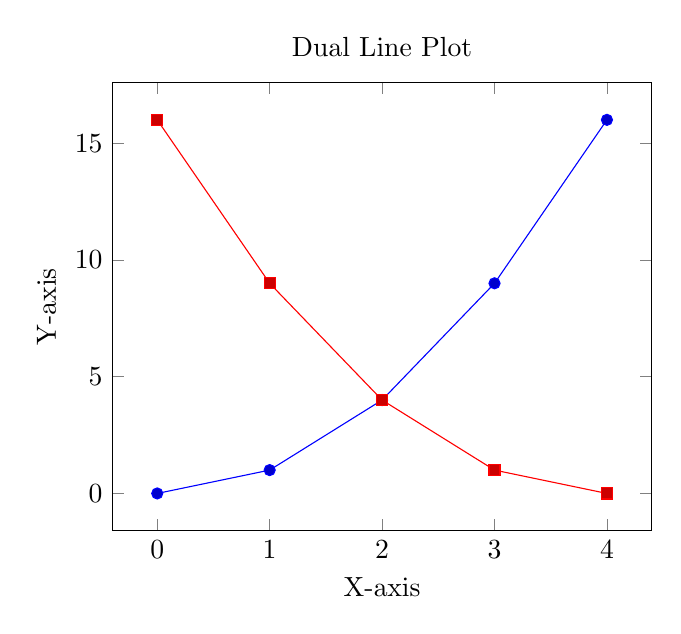
\begin{tikzpicture}
	\begin{axis}[
		title={Dual Line Plot},
		xlabel={X-axis},
		ylabel={Y-axis},
	]
		\addplot coordinates {
			(0,0)
			(1,1)
			(2,4)
			(3,9)
			(4,16)
		};
		\addplot coordinates {
			(0,16)
			(1,9)
			(2,4)
			(3,1)
			(4,0)
		};
	\end{axis}
\end{tikzpicture}
				\end{lstlisting}
				\caption{}
				\label{lst:line-plot-2}
			\end{subfigure}
			\hfill
			\begin{subfigure}[b]{0.45\linewidth}
				\centering
				\begin{tikzpicture}
					\begin{axis}[
						width=\linewidth,
						title={Dual Line Plot},
						xlabel={X-axis},
						ylabel={Y-axis},
					]
						\addplot coordinates {
							(0,0)
							(1,1)
							(2,4)
							(3,9)
							(4,16)
						};
						\addplot coordinates {
							(0,16)
							(1,9)
							(2,4)
							(3,1)
							(4,0)
						};
					\end{axis}
				\end{tikzpicture}
				\caption{}
				\label{plt:line-plot-2}
			\end{subfigure}
			\caption{A simple line plot with two sets of data.}
			\label{fig:line-plot-2}
		\end{figure}

	\section{Customizing Plots}
		This section provides some ways to increase the readability and customization of the plots we generate.
		\subsection{Adding a Legend}
			Legends can be added to plots for better readability.
			To add a legend to your plot you can use the code in \Cref{lst:legend-plot} to generate the plot shown in \Cref{fig:legend-plot}.
			Each plot is individually added to the legend by adding a \cmd{addlegendentry}\mopt{YOUR LEGEND ENTRY HERE} command following the \cmd{addplot} command.
			
			\note{The position of the legend can be specified by using the optional parameter \opt{legend pos=}} followed by a set of compass coordinates.
			
			\begin{lstlisting}[float=htbp,caption=,label=lst:legend-plot-header,style=LaTeXStyle,basicstyle=\small\ttfamily,]
\begin{figure}[H]
	\centering
	\begin{tikzpicture}
		\begin{axis}[
			title={Plot with Added Legend},
			xlabel={X-axis},
			ylabel={Y-axis},
			legend pos=north west,
		]
			\end{lstlisting}
			\begin{lstlisting}[float=htbp,caption=,label=lst:legend-plot-plots,style=LaTeXStyle,basicstyle=\small\ttfamily,]
			\addplot coordinates {
				(0,0)
				(1,1)
				(2,4)
				(3,9)
				(4,16)
			};
			\addlegendentry{\(y = x^2\)}
			\addplot coordinates {
				(0,16)
				(1,9)
				(2,4)
				(3,1)
				(4,0)
			};
			\addlegendentry{\(y = 16 - x^2\)}
		\end{axis}
	\end{tikzpicture}
	\caption{A customized plot with a legend.}
	\label{fig:legend-plot}
\end{figure}
		\end{lstlisting}
			\begin{figure}[H]
				\centering
				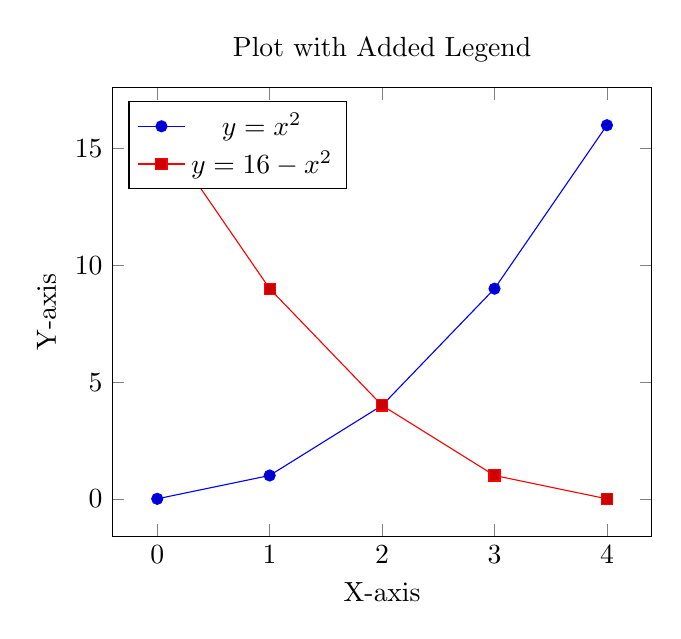
\begin{tikzpicture}
					\begin{axis}[
						title={Plot with Added Legend},
						xlabel={X-axis},
						ylabel={Y-axis},
						legend pos=north west,
					]
						\addplot coordinates {
							(0,0)
							(1,1)
							(2,4)
							(3,9)
							(4,16)
						};
						\addlegendentry{\(y = x^2\)}
						\addplot coordinates {
							(0,16)
							(1,9)
							(2,4)
							(3,1)
							(4,0)
						};
						\addlegendentry{\(y = 16 - x^2\)}
					\end{axis}
				\end{tikzpicture}
				\caption{A customized plot with a legend.}
				\label{fig:legend-plot}
			\end{figure}
		
		\subsection{Adding Grid Lines}
			To add gridlines to your plot 
			\begin{figure}[H]
				\centering
				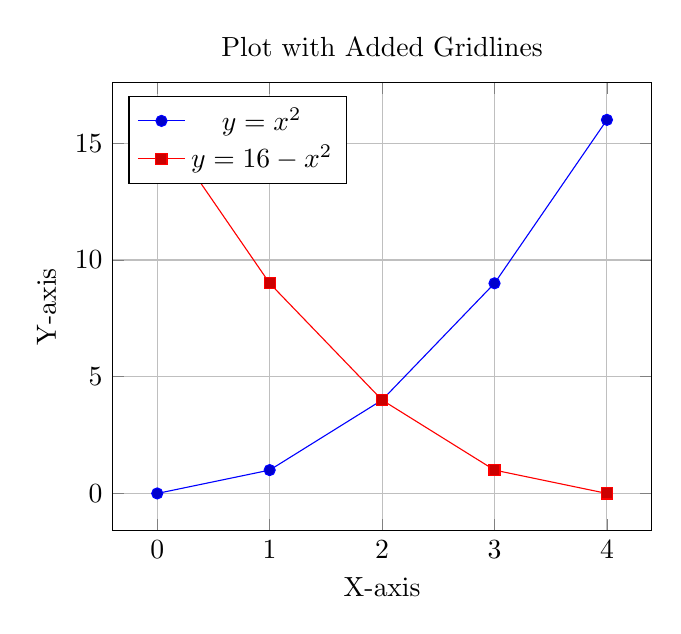
\begin{tikzpicture}
					\begin{axis}[
						title={Plot with Added Gridlines},
						xlabel={X-axis},
						ylabel={Y-axis},
						legend pos=north west,
						grid=major,
					]
						\addplot coordinates {
							(0,0)
							(1,1)
							(2,4)
							(3,9)
							(4,16)
						};
						\addlegendentry{\(y = x^2\)}
						\addplot coordinates {
							(0,16)
							(1,9)
							(2,4)
							(3,1)
							(4,0)
						};
						\addlegendentry{\(y = 16 - x^2\)}
					\end{axis}
				\end{tikzpicture}
				\caption{A customized plot with added gridlines.}
				\label{fig:gridlines-plot}
			\end{figure}

		\subsection{Changing Colors and Line Styles}
			Colors and line styles can be easily modified:

			\begin{figure}[H]
				\centering
				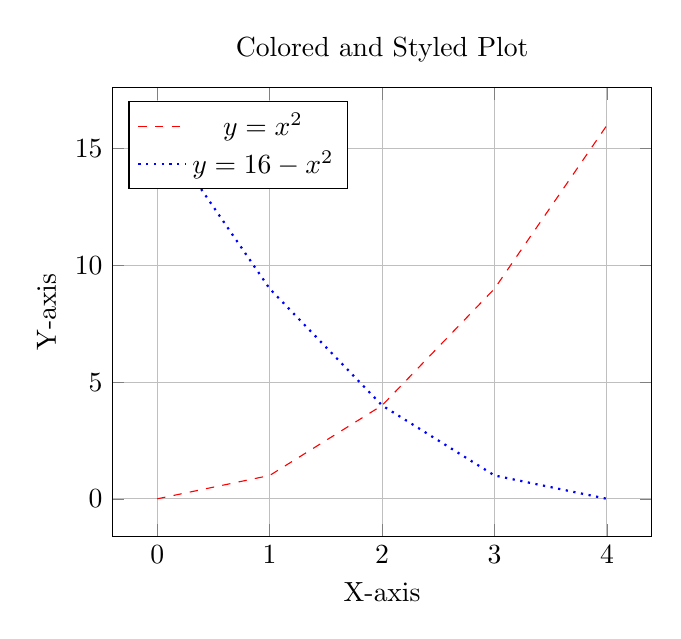
\begin{tikzpicture}
					\begin{axis}[
						title={Colored and Styled Plot},
						xlabel={X-axis},
						ylabel={Y-axis},
						legend pos=north west,
						grid=major,
					]
						\addplot[
							color=red,
							dashed
						] coordinates {
							(0,0)
							(1,1)
							(2,4)
							(3,9)
							(4,16)
						};
						\addlegendentry{\(y = x^2\)}
						\addplot[
							color=blue,
							thick,
							dotted
						] coordinates {
							(0,16)
							(1,9)
							(2,4)
							(3,1)
							(4,0)
						};
						\addlegendentry{\(y = 16 - x^2\)}
					\end{axis}
				\end{tikzpicture}
				\caption{A plot with customized colors and line styles}
				\label{fig:colour-plot}
			\end{figure}

	\section{Advanced Plot Types}
		\subsection{Equations}
			\begin{figure}[H]
				\centering
				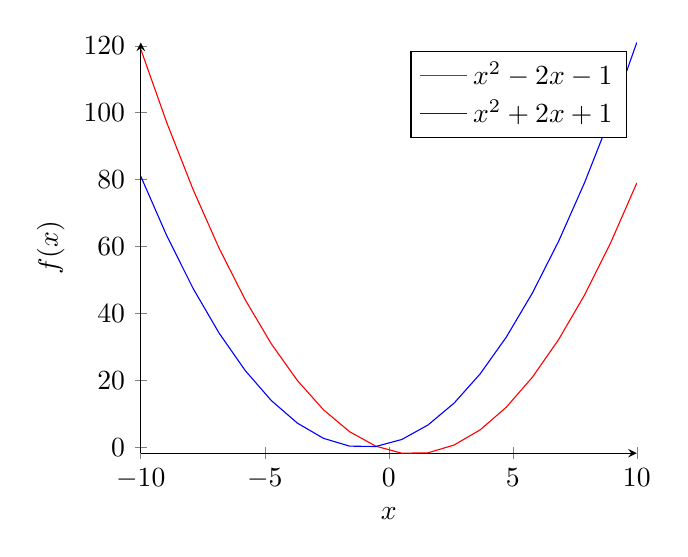
\begin{tikzpicture}
					\begin{axis}[
							width=0.65\linewidth,
							axis lines = left,
							xlabel = \(x\),
							ylabel = {\(f(x)\)},
						]
						\addplot[
								domain=-10:10, 
								samples=20, 
								color=red,
							]
							{x^2 - 2*x - 1};
						\addlegendentry{\(x^2 - 2x - 1\)}
						\addplot[
								domain=-10:10, 
								samples=20, 
								color=blue,
							]
							{x^2 + 2*x + 1};
						\addlegendentry{\(x^2 + 2x + 1\)}
					\end{axis}
				\end{tikzpicture}
				\caption{Plot of two parabola.}
				\label{fig:equation-plot}
			\end{figure}
		\subsection{Scatter Plot with External Data}
			\begin{figure}[H]
				\centering
				\begin{tikzpicture}
					\begin{axis}[
							width=0.65\linewidth,
							enlargelimits=true,
						]
						\addplot+[
								only marks,
								scatter,
								mark=*,
								mark size=2.9pt
							]
							table[meta=ma]
							{./99_Inclusions/Data/scattered_example.dat};
					\end{axis}
				\end{tikzpicture}
				\caption{Example of a Scatter Plot.}
				\label{fig:scatter-plot}
			\end{figure}
		\subsection{Bar Plot}
			Bar plots are useful for categorical data. 
			Here’s how to create one:
			\begin{figure}[H]
				\centering
				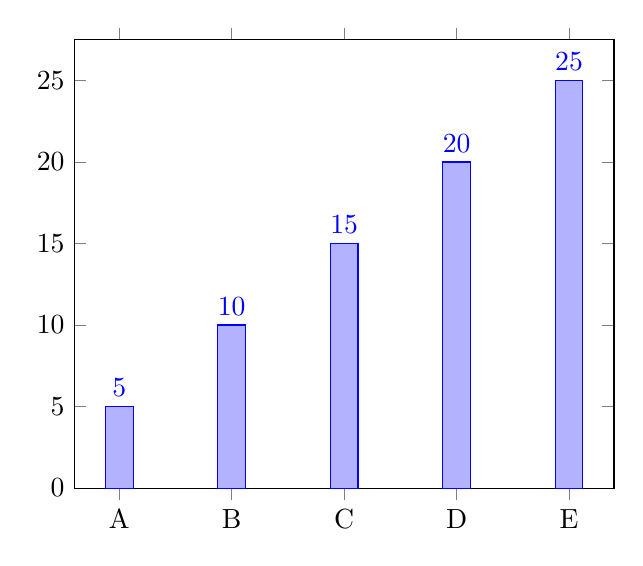
\begin{tikzpicture}
					\begin{axis}[
						ybar,
						symbolic x coords={A, B, C, D, E},
						xtick=data,
						nodes near coords,
						ymin=0,
					]
						\addplot coordinates {
							(A,5) (B,10) (C,15) (D,20) (E,25)
						};
					\end{axis}
				\end{tikzpicture}
				\caption{A bar plot}
				\label{fig:bar-plot}
			\end{figure}
			
			\begin{figure}[H]
				\centering
				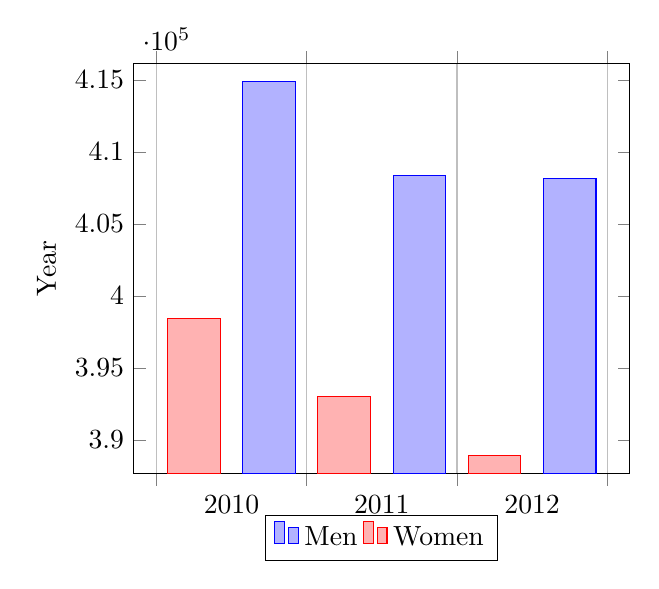
\begin{tikzpicture}
					\begin{axis}[
							width=0.65\linewidth,
							x tick label style={/pgf/number format/1000 sep=},
							ylabel=Year,
							enlargelimits=0.05,
							legend style={at={(0.5,-0.1)},
							anchor=north,legend columns=-1},
							ybar interval=0.7,
						]
						\addplot 
							coordinates {(2012,408184) (2011,408348)
							(2010,414870) (2009,412156)};
						\addplot 
							coordinates {(2012,388950) (2011,393007) 
							(2010,398449) (2009,395972)};
						\legend{Men,Women}
					\end{axis}
				\end{tikzpicture}
				\caption{Example of a Bar Graph.}
				\label{fig:bar-plot-2}
			\end{figure}
		
		\subsection{Pie Chart}
			Pie charts are less common in \LaTeX, but can still be created using the package \pkg{pgf-pie}:
			\begin{figure}[H]
				\centering
				\begin{tikzpicture}
					\pie[
						radius=2,
						text=legend,
					]{
						20/A, 30/B, 10/C, 25/D, 15/E
					}
				\end{tikzpicture}
				\caption{A basic pie chart.}
				\label{fig:pie-chart}
			\end{figure}
			
			\begin{figure}[H]
				\centering
				\begin{tikzpicture}
					\pie[
						radius=2,
						text=legend,
						explode={0, 0, 0, 0, 0.2},
					]{
						20/A, 30/B, 10/C, 25/D, 15/E
					}
				\end{tikzpicture}
				\caption{A pie chart with an ``Exploded'' slice.}
				\label{fig:pie-chart-2}
			\end{figure}
			
			\begin{figure}[H]
				\centering
				\begin{tikzpicture}
					\pie[
						square,
						text=legend,
					]{
						20/A, 30/B, 10/C, 25/D, 15/E
					}
				\end{tikzpicture}
				\caption{A ``square'' pie chart.}
				\label{fig:pie-chart-3}
			\end{figure}

		\subsection{3D Plot}
			3D plots can be created for more complex data visualization:
			\begin{figure}[H]
				\centering
				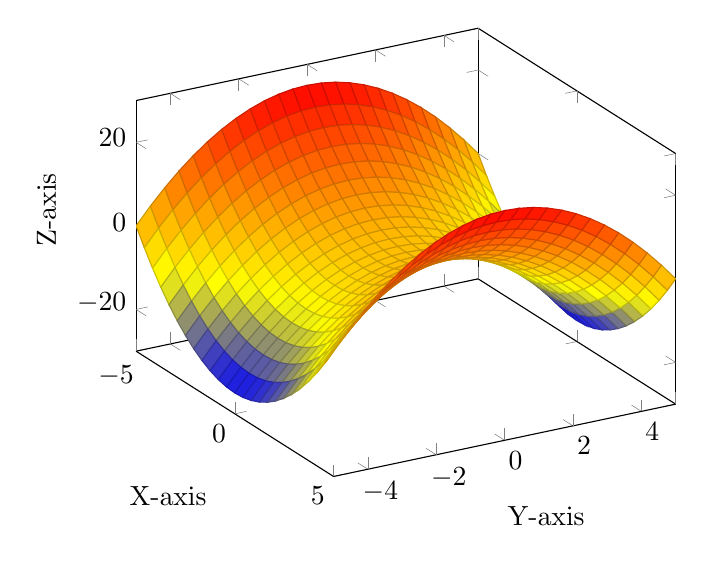
\begin{tikzpicture}
					\begin{axis}[
						view={60}{30},
						xlabel={X-axis},
						ylabel={Y-axis},
						zlabel={Z-axis},
					]
						\addplot3[surf] {
							x^2 - y^2
						};
					\end{axis}
				\end{tikzpicture}
				\caption{A 3D surface plot}
				\label{fig:3d-plot}
			\end{figure}
			
			\begin{figure}[H]
				\centering
				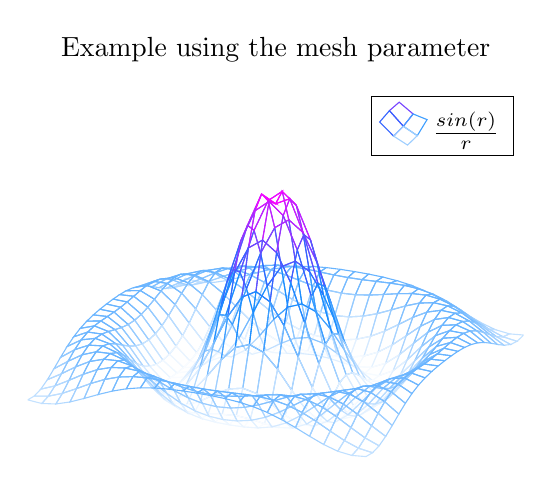
\begin{tikzpicture}
					\begin{axis}[
							width=0.65\linewidth,
							title=Example using the mesh parameter,
							hide axis,
							colormap/cool,
						]
						\addplot3[
								mesh,
								samples=25,
								domain=-8:8,
							]
							{sin(deg(sqrt(x^2+y^2)))/sqrt(x^2+y^2)};
						\addlegendentry{\(\frac{sin(r)}{r}\)}
					\end{axis}
				\end{tikzpicture}
				\caption{Example of a 3D Plot}
				\label{fig:3d-plot-2}
			\end{figure}

		\subsection{Polar Plot}
			Polar plots are useful for circular data:
			\begin{figure}[H]
				\centering
				\begin{tikzpicture}
					\begin{polaraxis}[
						title={Polar Plot},
						xlabel={Radius},
						ylabel={Angle (degrees)},
					]
						\addplot coordinates {
							(0,1) (30,2) (60,3) (90,4)
							(120,5) (150,6) (180,7)
						};
					\end{polaraxis}
				\end{tikzpicture}
				\caption{A polar plot}
				\label{fig:polar-plot}
			\end{figure}

		\subsection{Box Plot}
			Box plots are used to visualize the distribution of data:
			\begin{figure}[H]
				\centering
				\begin{tikzpicture}
					\begin{axis}[
						boxplot/draw direction=y,
						x axis line style = {opacity=0},
						axis x line* = bottom,
						axis y line = left,
						ymajorgrids,
						ytick = {0, 5, 10},
						ylabel={Values},
						ymin=0,
						ymax=10,
						enlarge y limits,
						xtick = {1, 2},
						xticklabel style = {align=center, font=\small, rotate=60},
						xticklabels = {Apples, Oranges},
					]
						\addplot+[
							boxplot prepared={
								median=5,
								upper quartile=6,
								lower quartile=4,
								upper whisker=7,
								lower whisker=3
							},
							color=blue
						] coordinates {};
						\addplot+[
							boxplot prepared={
								median=4,
								upper quartile=5,
								lower quartile=2,
								upper whisker=8,
								lower whisker=1
							},
							color=red
						] coordinates {};
					\end{axis}
				\end{tikzpicture}
				\caption{A box plot}
				\label{fig:box-plot}
			\end{figure}

	\section{Conclusion}
		The \pkg{pgfplots} package is an incredibly versatile tool for creating a wide range of plots and graphs in \LaTeX. 
		This chapter has provided examples of various plot types and customization options, showcasing the power and flexibility of \pkg{pgfplots}. 
		By leveraging these capabilities, you can create high-quality, publication-ready figures for your thesis.